\documentclass{../../slides-style}

\slidetitleext[Часть 1]{Лекция 6: Управление проектами, риски и оценка}{26.03.2024}{Управление проектами}

\begin{document}

    \begin{frame}[plain]
        \titlepage
    \end{frame}

    \section{Функции менеджера проекта}

    \begin{frame}
        \frametitle{Факторы успеха проектов}
        \begin{itemize}
            \item Соглашение между ключевыми участниками о целях проекта
            \item Управляемые границы проекта
            \item План как средство отслеживания прогресса
            \item Правильные люди на правильных местах
            \item Эффективные коммуникации
        \end{itemize}
    \end{frame}

    \begin{frame}
        \frametitle{Функции менеджера проекта}
        \begin{center}
            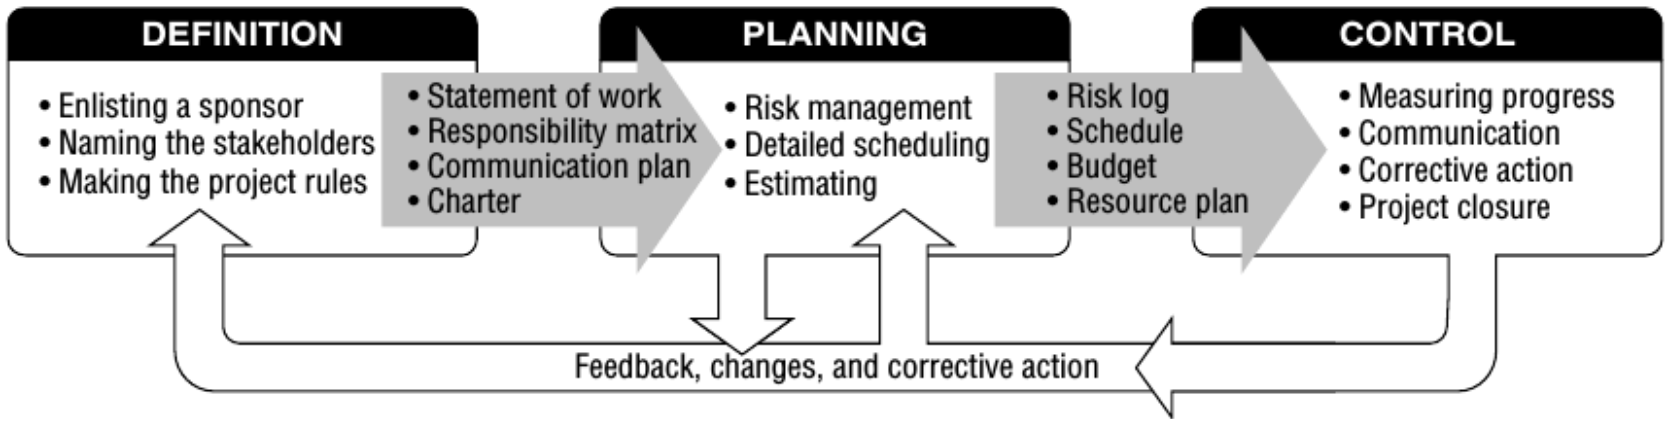
\includegraphics[width=0.9\textwidth]{projectManagerFunctions.png}
        \end{center}
    \end{frame}

    \section{Заинтересованные лица}

    \begin{frame}
        \frametitle{Stakeholder roles (заинтересованные субъекты)}
        \begin{itemize}
            \item Менеджер проекта
            \item Команда
            \begin{itemize}
                \item Ключевые
                \item Вспомогательные
                \item Подрядчики
                \item Пользователи, заказчики
            \end{itemize}
            \item Менеджмент
            \begin{itemize}
                \item Высшее руководство
                \item Другие менеджеры направлений/отделов/проектов
                \item Спонсор/попечитель/покровитель проекта
            \end{itemize}
            \item Заказчики
        \end{itemize}
    \end{frame}

    \begin{frame}
        \begin{center}
            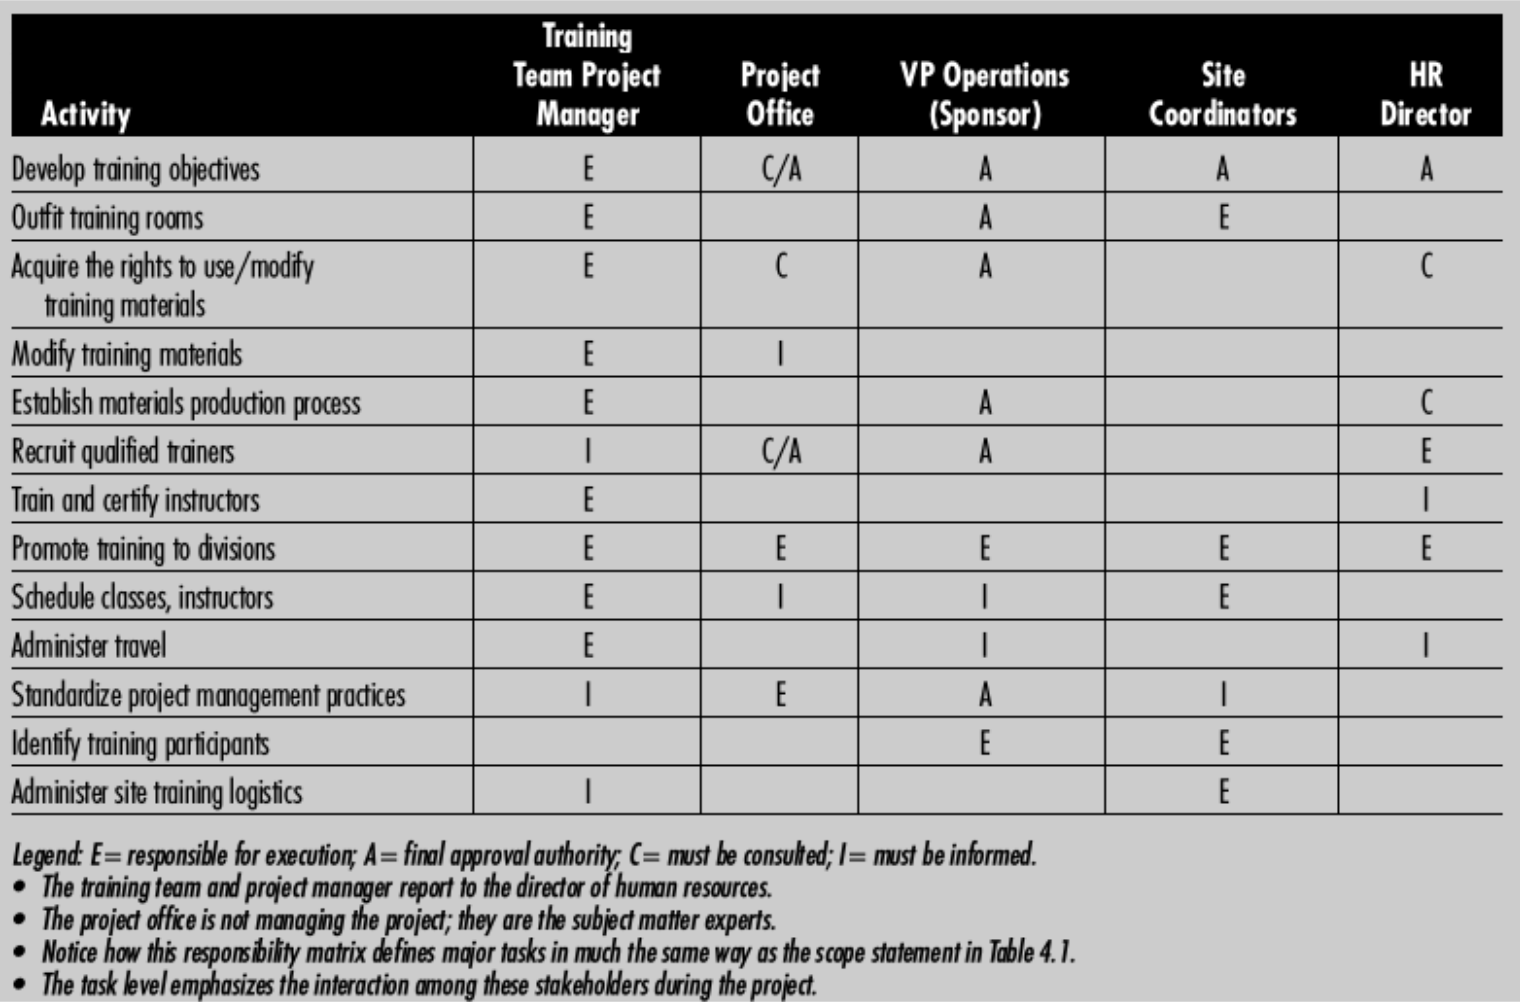
\includegraphics[width=0.9\textwidth]{stakeholders.png}
        \end{center}
    \end{frame}

    \section{План коммуникаций}

    \begin{frame}
        \frametitle{План коммуникаций}
        \begin{itemize}
            \item Нужная информация нужным людям в нужное время
            \begin{itemize}
                \item Какие именно люди?
                \item Какая конкретно информация?
                \begin{itemize}
                    \item Тип (подтверждения, отчёты о прогрессе, координация, …)
                    \item Объём
                \end{itemize}
                \item В какой момент времени?
                \item Каков способ коммуникации?
            \end{itemize}
            \item Механизмы делегирования и эскалации
        \end{itemize}
    \end{frame}

    \begin{frame}
        \begin{center}
            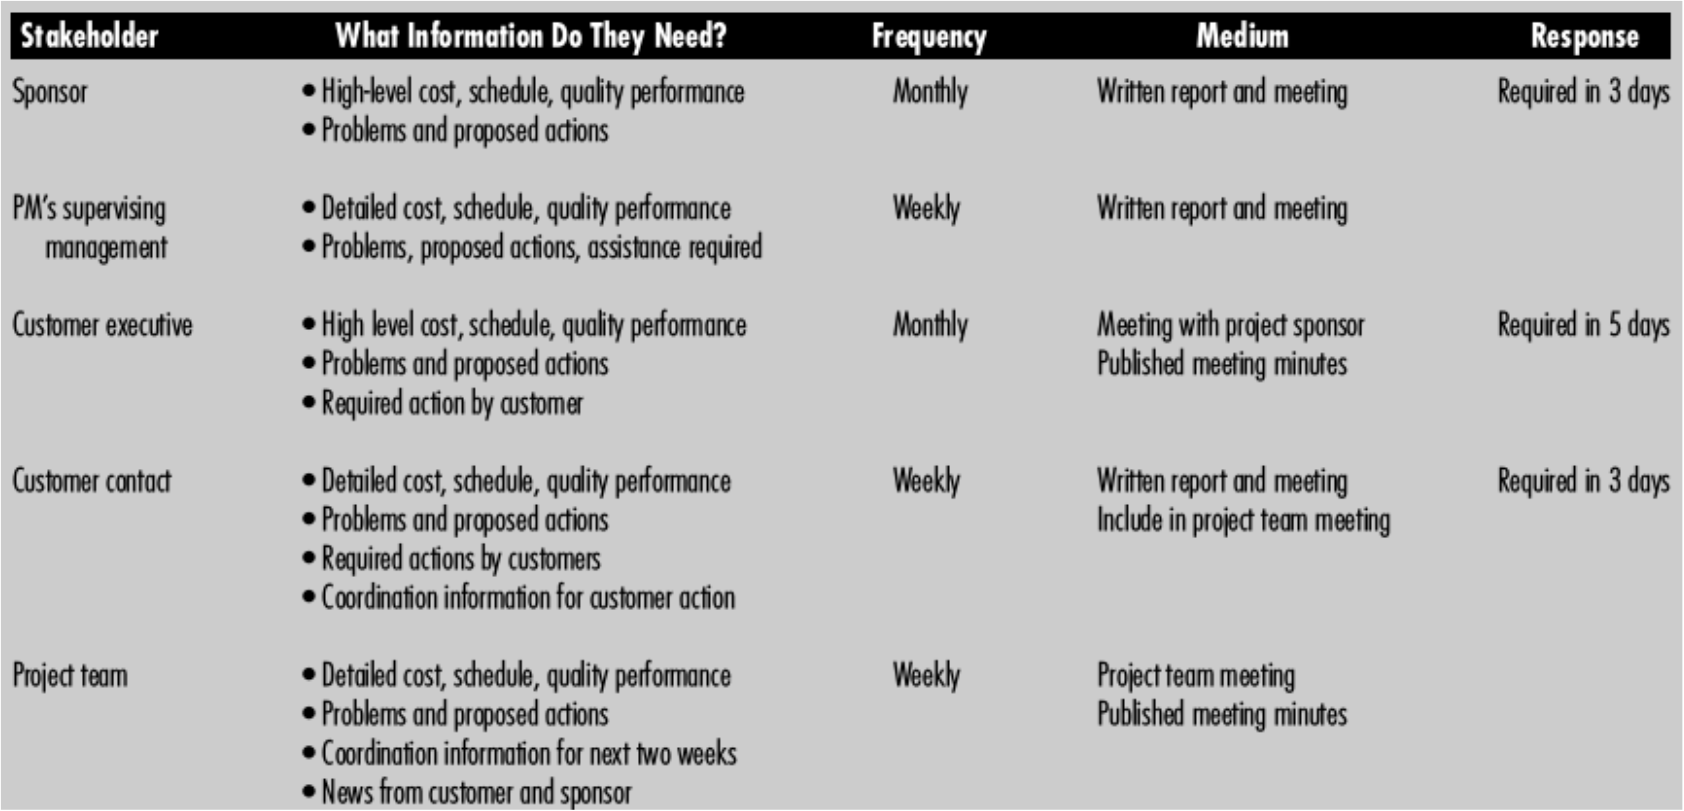
\includegraphics[width=0.9\textwidth]{communicationPlan.png}
        \end{center}
    \end{frame}

    \section{Планирование}

    \begin{frame}
        \frametitle{Планирование}
        \begin{columns}
            \begin{column}{0.3\textwidth}
                \begin{itemize}
                    \item Что?
                    \item Почему/зачем?
                    \item Когда?
                    \item Как?
                    \item Где?
                    \item Кто?
                \end{itemize}
            \end{column}
            \begin{column}{0.7\textwidth}
                \begin{center}
                    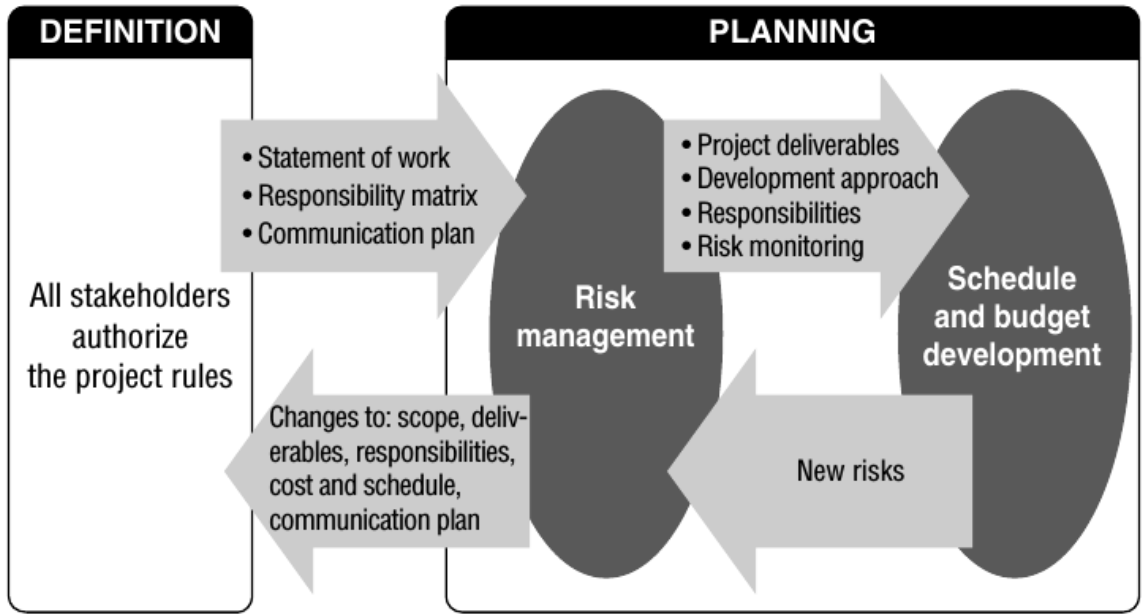
\includegraphics[width=0.9\textwidth]{planning.png}
                \end{center}
            \end{column}
        \end{columns}
    \end{frame}

    \section{Управление рисками}

    \begin{frame}
        \frametitle{Управление рисками}
        \begin{columns}
            \begin{column}{0.6\textwidth}
                \begin{itemize}
                    \item Риск = неопределённость + неприятный исход
                    \begin{itemize}
                        \item Известное неизвестное
                        \item Неизвестное неизвестное
                    \end{itemize}
                    \item Управление рисками --- первоочередная задача менеджера проекта
                \end{itemize}
            \end{column}
            \begin{column}{0.4\textwidth}
                \begin{center}
                    
\includegraphics[width=0.7\textwidth]{riskManagement.png}
                \end{center}
            \end{column}
        \end{columns}
    \end{frame}

    \begin{frame}
        \begin{center}
            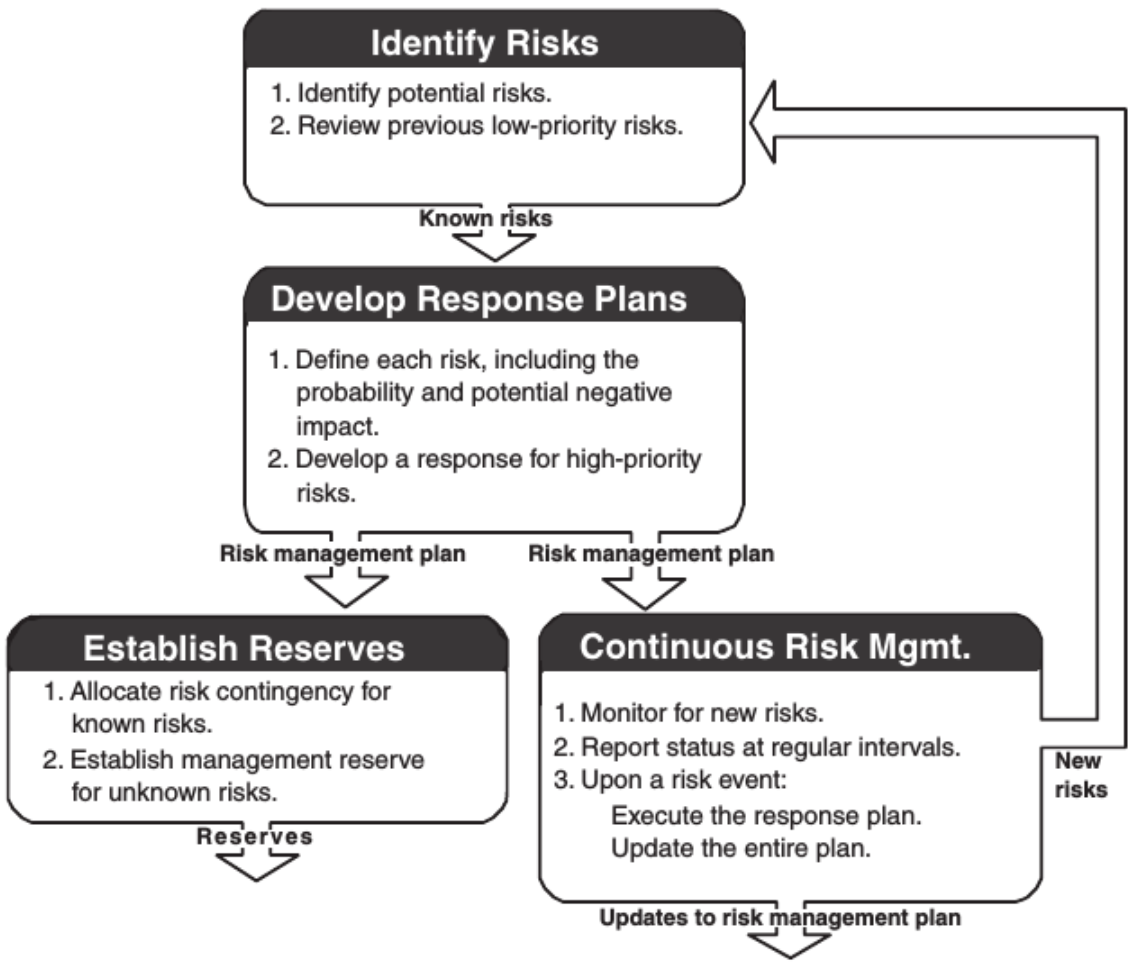
\includegraphics[width=0.7\textwidth]{riskManagementLoop.png}
        \end{center}
    \end{frame}

    \begin{frame}
        \frametitle{Шаг 1: идентификация рисков}
        \begin{itemize}
            \item Получение информации от stakeholder’ов
            \begin{itemize}
                \item Мозговые штурмы
                \item Интервью
            \end{itemize}
            \item Использование прошлого опыта
            \begin{itemize}
                \item Построение профиля рисков
                \item анализ аналогичных проектов
            \end{itemize}
            \item Риски графика работ и бюджета
        \end{itemize}
    \end{frame}

    \begin{frame}
        \frametitle{Шаг 2: разработка стратегии противодействия}
        \begin{itemize}
            \item Определение серьёзности риска
            \begin{itemize}
                \item Описание условий возникновения и последствий
            \end{itemize}
            \item Определение вероятности возникновения
            \begin{itemize}
                \item Количественные оценки
                \item Субъективная качественная оценка
            \end{itemize}
            \item Определение стратегии снижения возможного урона от риска
            \begin{itemize}
                \item Принять
                \item Избежать
                \item Переложить на кого-то другого
                \item Смягчить
                \item Отслеживать
                \begin{itemize}
                    \item Отслеживаемость риска
                    \item события-триггеры
                \end{itemize}
            \end{itemize}
        \end{itemize}
    \end{frame}

    \begin{frame}
        \begin{center}
            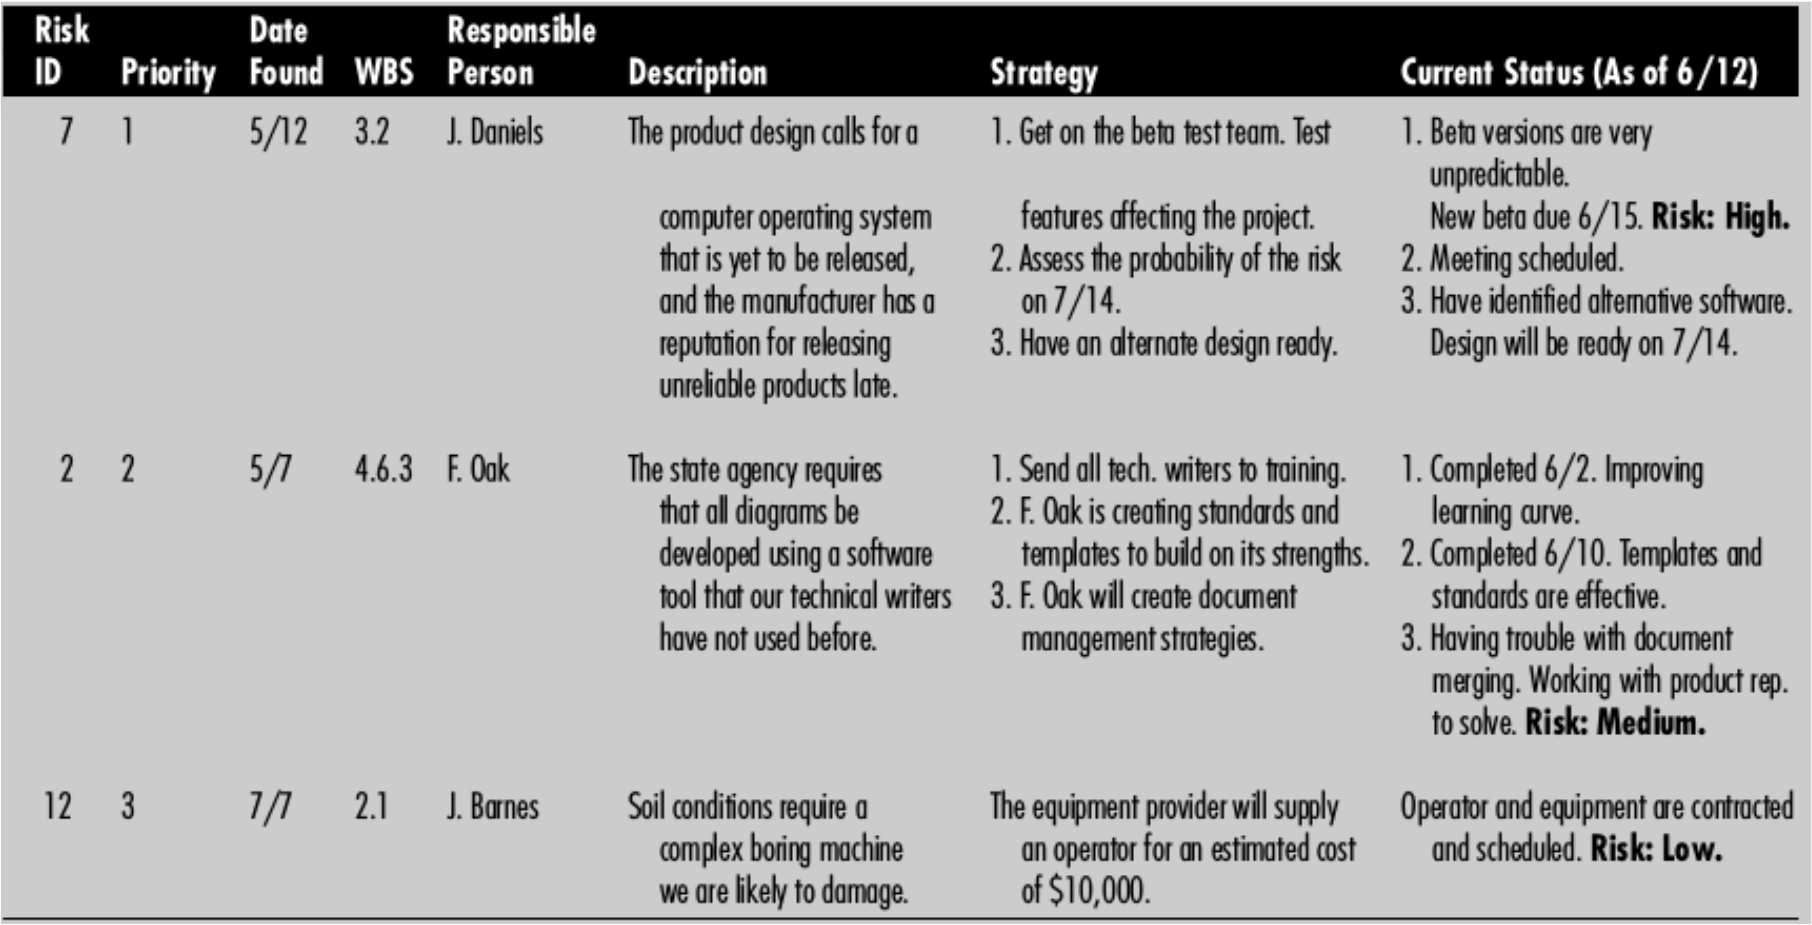
\includegraphics[width=\textwidth]{riskExample.png}
        \end{center}
    \end{frame}

    \begin{frame}
        \begin{center}
            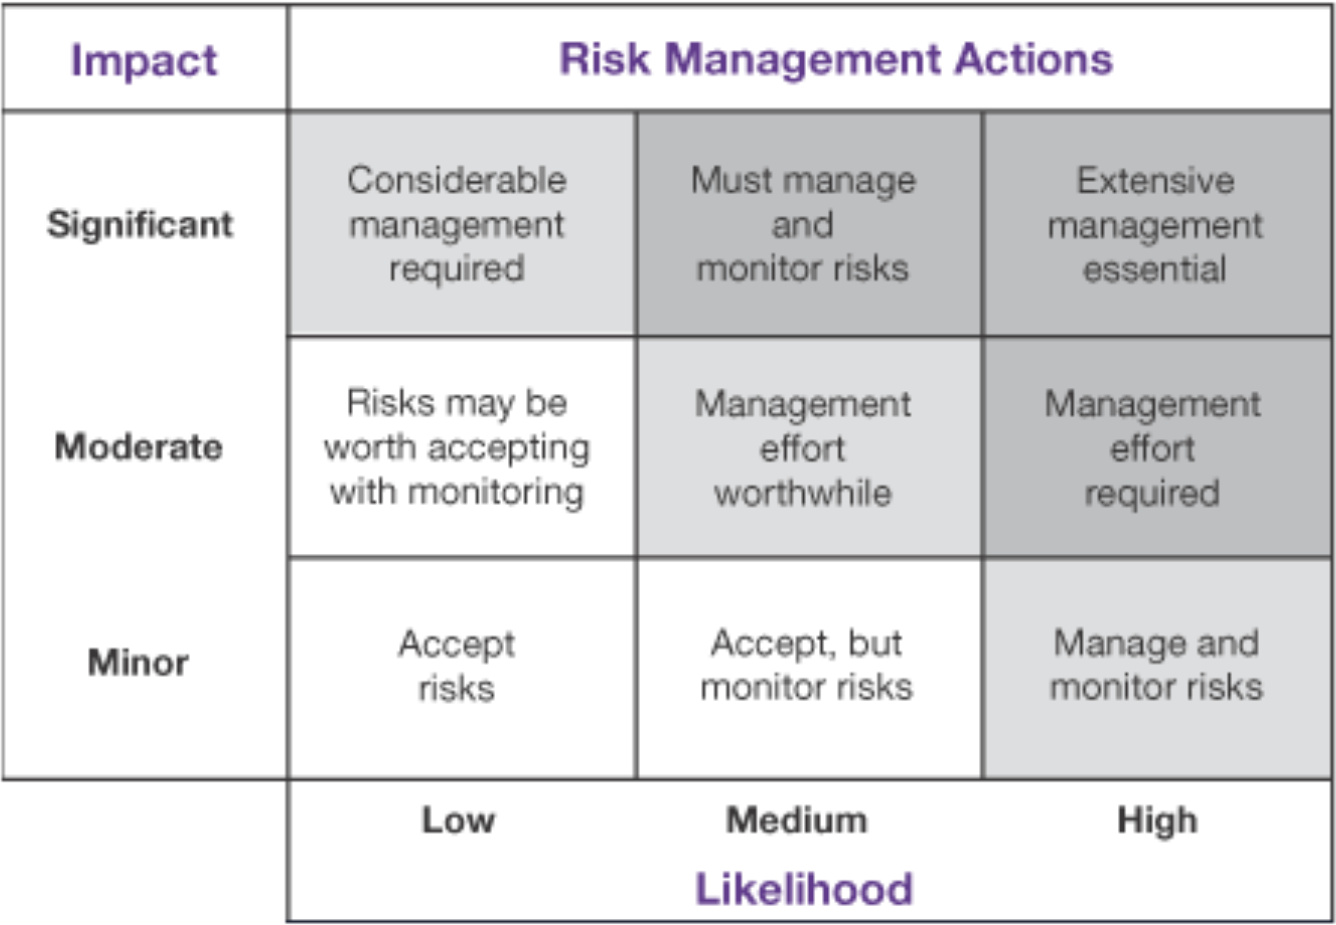
\includegraphics[width=0.6\textwidth]{riskMatrix.png}
        \end{center}
    \end{frame}

    \begin{frame}
        \frametitle{Шаг 3: Создать резервный фонд}
        \begin{itemize}
            \item Противодействие известным рискам
            \begin{itemize}
                \item Определить План Б для каждого отслеживаемого риска
                \item Оценить стоимость Плана Б для каждого риска
                \item Умножить на вероятности и сложить
                \item Согласовать ``разумный'' бюджет
            \end{itemize}
            \item А ещё есть неизвестное неизвестное!
            \begin{itemize}
                \item +5-30\% бюджета в зависимости от типа проекта
            \end{itemize}
        \end{itemize}
    \end{frame}

    \begin{frame}
        \frametitle{Шаг 4: Непрерывное управление рисками}
        \begin{itemize}
            \item Поддержание списка рисков
            \item Запланированные переоценки известных рисков
            \item Поиск информации, поиск новых рисков
            \item Анализ резервного фонда
        \end{itemize}
    \end{frame}

    \section{Декомпозиция проекта}

    \begin{frame}
        \frametitle{Декомпозиция проекта}
        \begin{itemize}
            \item Визуализация границ проекта
            \item Отслеживание прогресса
            \item Оценка стоимости и графика проекта
            \item Организация работы команды
        \end{itemize}
    \end{frame}

    \begin{frame}
        \begin{center}
            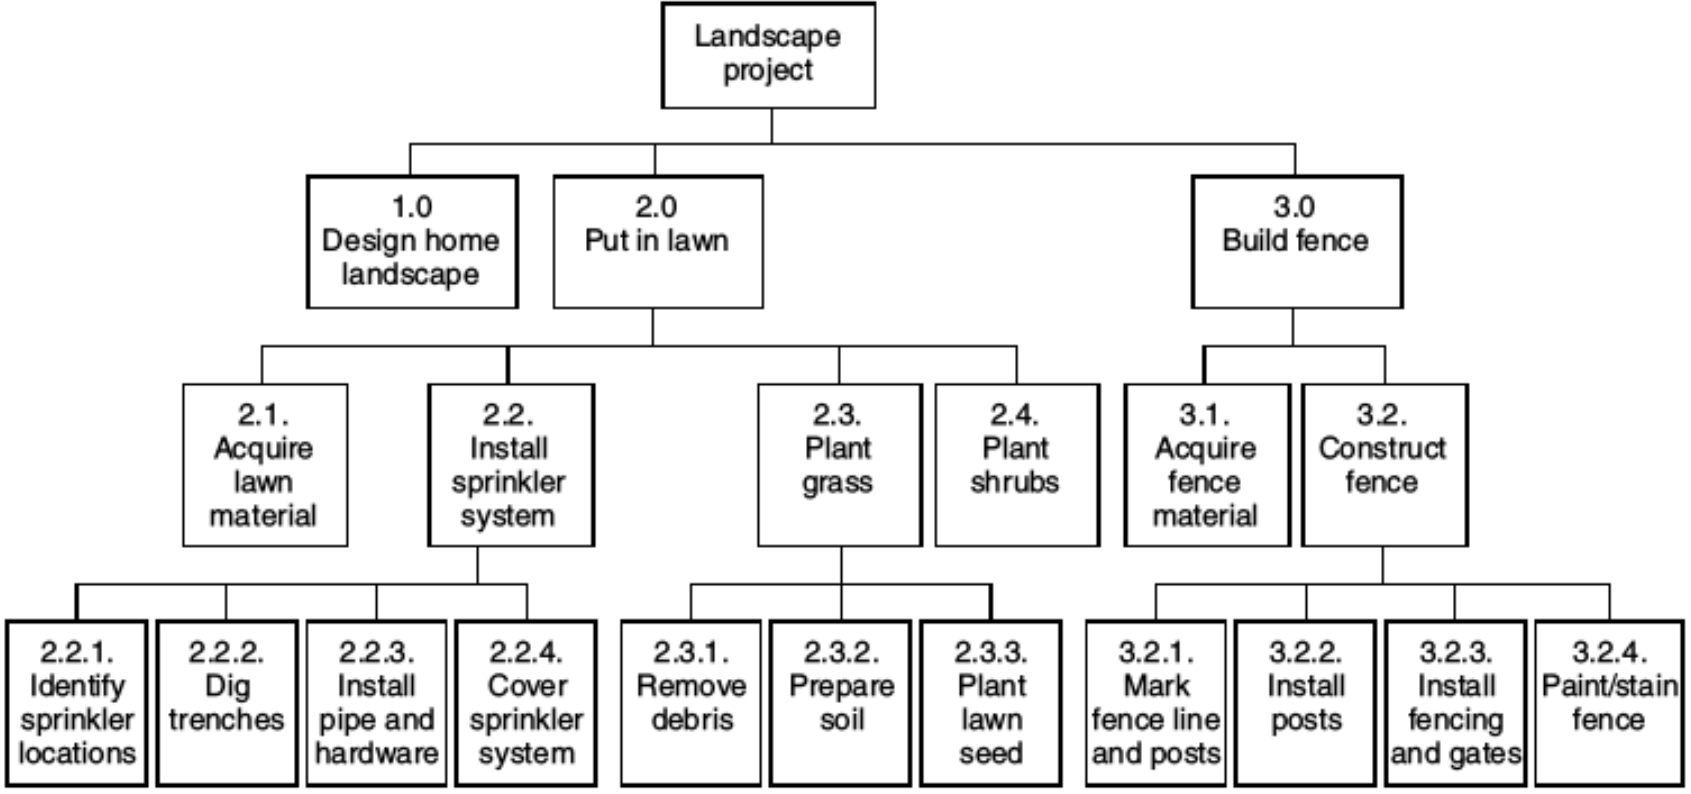
\includegraphics[width=\textwidth]{wbsExample.png}
        \end{center}
    \end{frame}

    \begin{frame}
        \begin{center}
            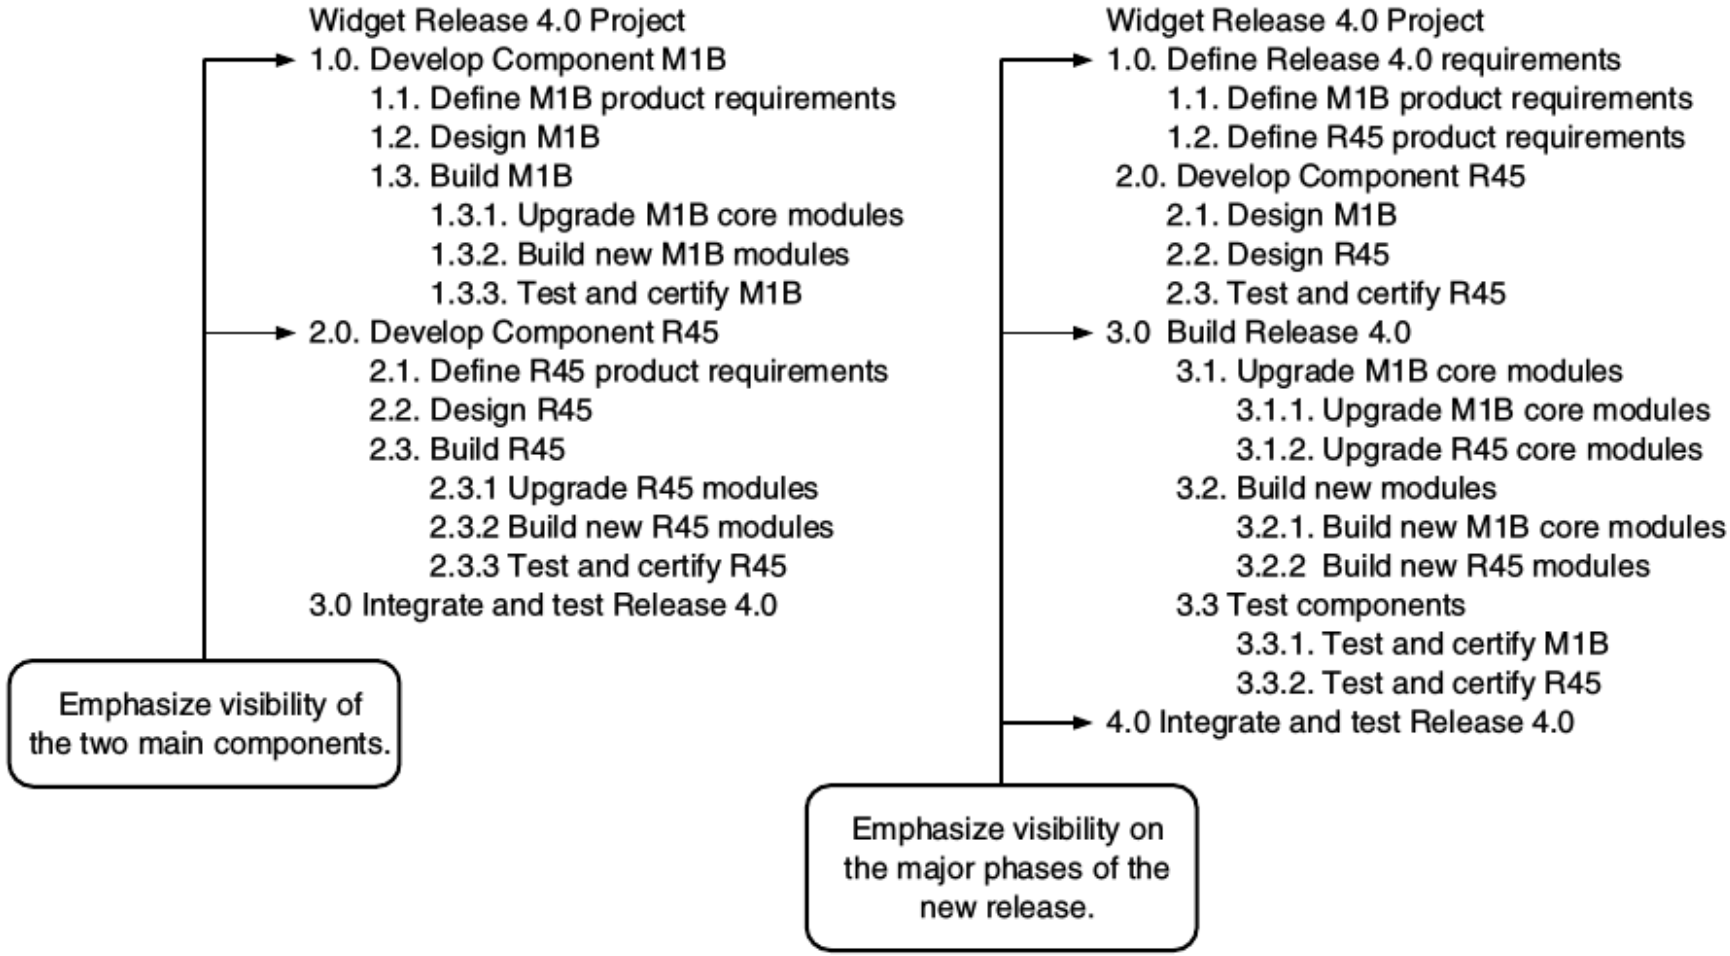
\includegraphics[width=0.9\textwidth]{wbsExample2.png}
        \end{center}
    \end{frame}

    \begin{frame}
        \frametitle{Критерии хорошей декомпозиции}
        \begin{itemize}
            \item Не TODO --- требуются отчуждаемые артефакты
            \item Полнота разбиения задач
            \begin{itemize}
                \item На всех уровнях сумма объёма дочерних работ в точности равна объёму работы дочернего узла
                \item Отдельные работы друг с другом не пересекаются
            \end{itemize}
            \item Понятность и конкретность задач
            \begin{itemize}
                \item Явный вид деятельности
                \item Явный результат
            \end{itemize} 
        \end{itemize}
    \end{frame}

    \begin{frame}
        \frametitle{Критерии SMART}
        \begin{itemize}
            \item Specific --- задача должна быть конкретной
            \begin{itemize}
                \item И однозначно пониматься всеми участниками
            \end{itemize}
            \item Measurable --- задача должна быть измеримой
            \begin{itemize}
                \item KPI, желательно числовые
            \end{itemize}
            \item Achievable --- задача должна быть достижимой 
            \begin{itemize}
                \item Реальные сроки
                \item Опираться на объективные показатели (предыдущий опыт, средние показатели)
            \end{itemize}
            \item Relevant --- задача должна быть значимой
            \begin{itemize}
                \item Укладываться в общую стратегию проекта
            \end{itemize}
            \item Time bound --- задача должна быть ограниченной по времени
            \begin{itemize}
                \item Правило 8/80
            \end{itemize}
        \end{itemize}
    \end{frame}

    \begin{frame}
        \frametitle{Размер конечных задач}
        \begin{itemize}
            \item Правило 8/80
            \item Привязка к периодам отчётности
            \item Здравый смысл
            \begin{itemize}
                \item Простота оценки, реализации, контроля
                \item Сложность проектирования, интеграции, микроменеджмент
            \end{itemize} 
        \end{itemize}
    \end{frame}

    \begin{frame}
        \frametitle{Учёт задач по управлению проектом}
        \begin{center}
            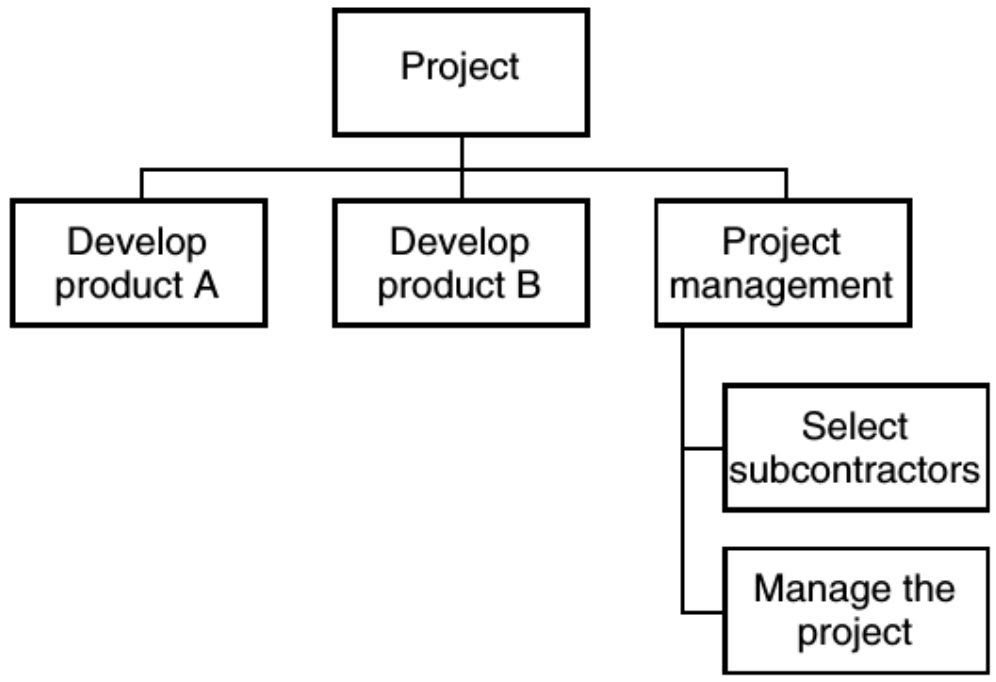
\includegraphics[width=0.6\textwidth]{wbsProjectManagementTasks.png}
        \end{center}
    \end{frame}

    \begin{frame}
        \frametitle{Как делать}
        \begin{enumerate}
            \item Собрать все важные документы
            \begin{itemize}
                \item Требования, информация по отчуждаемым артефактам и т.д.
            \end{itemize}
            \item Определить ключевых участников команды
            \item Определить элементы 1 уровня
            \begin{itemize}
                \item Использовать фазовый или артефактный подход?
                \item Правило 100\%
            \end{itemize}
            \item Рекурсивно повторить шаг 3 для каждого элемента 1 уровня
            \item Создать словарь WBS
            \begin{itemize}
                \item Описание работы в каждом блоке, границы, этапы, риски, стоимость и т.д.
            \end{itemize}
            \item Составить диаграмму Гантта/сетевой график
        \end{enumerate}
    \end{frame}

\end{document}
